\documentclass{iacrtrans}
\usepackage[utf8]{inputenc}

% -- Better auto-referencing --
\usepackage{hyperref}
\usepackage[nameinlink]{cleveref}
\crefname{algocf}{alg.}{algs.}
\Crefname{algocf}{Algorithm}{Algorithms}

% -- Some neat table packages --
\usepackage{makecell}
\usepackage{arydshln}
\usepackage{siunitx} % For group separators when writing long integers

% -- Algorithms --
\usepackage[
    titlenumbered,
    linesnumbered,
    ruled
]{algorithm2e}
\SetKwInOut{Input}{Input}
\SetKwInOut{Output}{Output}
\SetKwInOut{Return}{Return}

\SetKwComment{Comment}{/* }{ */}
\newcommand\mycommentstyle[1]{\footnotesize\ttfamily\textcolor{red!70!black}{#1}}
\SetCommentSty{mycommentstyle}

% -- Setting format for equations --
\usepackage{xcolor}
\usepackage{empheq}

\usepackage[most]{tcolorbox}

\newtcolorbox{empheqboxed}{%
  enhanced,
  boxsep=1pt,
  arc=0.75ex,
  colback=gray!10,
  colframe=gray!40,
  boxrule=1pt,
  leftrule=40pt,
  top=-3.5mm,
  overlay unbroken and first ={%
    \node[minimum width=1cm,
          anchor=south,
          font=\sffamily\bfseries,
          xshift=20pt,
          yshift=-6.5pt,
          black]
    at (frame.west) {Stack:};
  }
}

% -- Bitcoin Script Commands --
\newcommand{\elem}[1]{\, \langle #1 \rangle \,}
\newcommand{\opcode}[1]{\, \texttt{#1} \,}
\newcommand{\script}[1]{ $\big\{ #1 \big\}$ }

\author{Dmytro Zakharov\inst{1} \and Oleksandr Kurbatov\inst{1} \and Manish Bista\inst{2} \and Belove Bist\inst{2}}
\institute{Research Department at Distributed Lab \email{dmytro.zakharov@distributedlab.com}, \email{ok@distributedlab.com}\and Alpen Labs \email{manish@alpenlabs.io }, \email{belove@alpenlabs.io}}
\title[Fast Multiplication on Bitcoin]{Fast Big Integer Multiplication using $w$-windowed method on Bitcoin}

\begin{document}

\maketitle

% use optional argument because the \LaTeX command breaks the PDF keywords
\keywords[]{Bitcoin, Bitcoin Script, Fast Multiplication, Elliptic Curve Scalar Multiplication, BitVM}

\begin{abstract}
    A crucial component of any SNARK system is performing finite field arithmetic, which inherently involves the fundamental task of multiplying two large integers. Performing such arithmetic on Bitcoin is particularly challenging due to the limitations of Bitcoin's scripting language. Bitcoin Script is intentionally non-Turing-complete and stack-based, designed with simplicity and security in mind. Hence, it lacks built-in support for complex arithmetic operations and has constraints on the size and number of stack elements. Implementing efficient big integer multiplication requires innovative techniques to work within these constraints while minimizing the number of opcodes used.
    
    This paper introduces the $w$-windowed method for multiplying two 254-bit prime $q$ (BN254 curve) integers, along with additional optimization techniques. Building on this fast multiplication, we implement modular multiplication with further enhancements. Our approach significantly reduces the number of opcodes compared to state-of-the-art methods, making it a substantial improvement in performing finite field arithmetic on Bitcoin. This primitive, central to protocols like SNARKnado, brings us closer to practical SNARK verification on Bitcoin.
\end{abstract}

\tableofcontents{}

\section{Introduction}

% To be done

\section{Preliminaries}

\subsection{Bitcoin Script}

\subsubsection{Basic Structure}
\textbf{Bitcoin Script} is a stack-based, not Turing-complete language used for specifying conditions on how UTXO can be spent \cite{mastering_bitcoin}. Informally, this condition is called \texttt{scriptPubKey}, while the data that must be provided to meet this condition is called \texttt{scriptSig}\footnote{Formally, \texttt{scriptSig} might contain the logic as well, but we omit the details here.}. To verify that the condition is met based on \texttt{scriptSig} provided, one should first concatenate $\texttt{scriptSig} \parallel \texttt{scriptPubKey}$, execute the script and verify that the resultant stack contains a non-false value (meaning, anything except for \texttt{0}). 

The stack consists of the values placed in the script and the so-called \textbf{opcodes} --- keywords that operate with the elements in the stack. Let us consider some examples to introduce notation and describe how the script gets executed. 

\textbf{Example 1.} The script \script{\elem{a} \elem{b} \opcode{OP\_ADD} \elem{c} \opcode{OP\_EQUAL}} verifies whether given $a,b,c$ satisfy $a+b=c$. We first push two integers $a$ and $b$ to the stack, then \texttt{OP\_ADD} will consume $a$ and $b$ (meaning, they get removed) and output $s \gets a+b$, so the stack becomes \script{\elem{s} \elem{c} \opcode{OP\_EQUAL}}. Finally, \texttt{OP\_EQUAL} takes $s$ and $c$ and outputs \texttt{OP\_TRUE} if $a+b=c$, and \texttt{OP\_FALSE}, otherwise. Note that such notation is commonly called the \textit{Reverse Polish Notation} in the literature \cite{reverse_polish_notation}.

\textbf{Example 2.} Suppose our condition on spending the coins is providing the pre-image of the given hash value $h$ (that is, providing a message $m$ such that $h = \mathsf{H}(m)$), which is called the \textit{Hashlock Script}. In this case, our \texttt{scriptPubKey} looks as follows\footnote{It should be noted, though, that in the placeholder $\langle h \rangle$ we should push \texttt{0x20} followed by 20 bytes of $h$.}:
\begin{empheqboxed}
\begin{align*}
    \opcode{OP\_HASH160} \elem{h} \opcode{OP\_EQUAL}
\end{align*}
\end{empheqboxed}

Suppose we brought a message $m$, our \texttt{scriptSig}. Concatenating \texttt{scriptSig} and \texttt{scriptPubKey} would result in the following script:
\begin{empheqboxed}
\begin{align*}
    \elem{m} \opcode{OP\_HASH160} \elem{h} \opcode{OP\_EQUAL}
\end{align*}
\end{empheqboxed}

Execution in this case would proceed as follows:
\begin{enumerate}
    \item First, $m$ is added to the stack.
    \item Next, \texttt{OP\_HASH160} will hash the provided value $h' \gets \mathsf{H}(m)$, so the stack would become \script{\elem{h'} \elem{h} \opcode{OP\_EQUAL}}.
    \item Finally, after executing \texttt{OP\_EQUAL}, we will either get \texttt{OP\_TRUE} on the top of the stack if $h = h'$, or \texttt{OP\_FALSE} otherwise. 
\end{enumerate}

Note that we get \texttt{OP\_TRUE} (meaning, we can spend the coins) only if $h'=h$ or, equivalently, $\mathsf{H}(m)=h$, what was needed from the start.

\subsubsection{Arithmetic in Bitcoin}\label{section:arithmetic_bitcoin}

To implement the SNARK verifier on Bitcoin, one must implement the finite field arithmetic over the elliptic curve scalar field $\mathbb{F}_q$. The bitsize of such scalar field is typically from $254$ bits (as for \textit{BN254} \cite{bn254}) to $381$ bits and more (as for \textit{BLS12-381} \cite{bls12}). Currently, the common choice is the \textit{BN254} based on $254$-bit prime order $q$, which, for example, is currently used for elliptic curve precompiles in \textit{Ethereum} \cite{ethereum}. Although further discussion is valid for any fairly large $q$, our implementation was focused on $254$-bit $q$. 

Finite field arithmetic over $N$-bit $q$ (where $N=254$ for \textit{BN254}, for example) includes implementing the widening multiplication of two $N$-bit numbers, resulting in a $2N$-bit integer. Why is this a problem in Bitcoin at all? The main issue is that Bitcoin does not have a multiplication opcode\footnote{At some point, Bitcoin did have \texttt{OP\_MUL}, but it was later disabled.}. To make matters worse, integers on the stack are 32-bit, meaning that representing large integers requires some additional workload. Therefore, we will use the \textbf{base $\beta$} representation of an integer.

\begin{definition}
    Given positive integer $x \in \mathbb{Z}_{\geq 0}$, \textbf{base $\beta$} representation is an expression
    \begin{equation}
        x = \sum_{k=0}^{\ell-1}x_k \times\beta^k,
    \end{equation}
    where each \textbf{limb} $x_k$ is between $0$ and $\beta-1$, and $\ell$ is the length of such representation. We further denote such representation by $(x_0,x_1,\dots,x_{\ell-1})_{\beta}$. 
\end{definition}

Empirically, it seems that using larger bases results in smaller scripts. The main reason is that larger bases result in the shorter representation of integers. However, this does not mean better methods with shorter integers will not produce shorter scripts in the future. Therefore, we pick $\beta=2^{30}$: it is the power of two, which would come in handy later, and we will not run out of 32 bits when performing arithmetic (doublings, additions, etc.). Also, assume the limb size in bits is $n=30$.

Moreover, Bitcoin does not have loops (recall that Bitcoin Script is not Turing complete!), meaning that the length of our representation must be fixed. It means that $\ell = \lceil N/n \rceil$, or, $\ell=9$ in our particular case. 

All things combined, \Cref{alg:integer_representation} shows how to preprocess the given integer $x$ and push the representation to the stack.

\begin{algorithm}
\caption{Pushing given integer to the stack}\label{alg:integer_representation}
\Input{Integer $x$ of bit size up to $N$}
\Output{Representation $(X_0,X_1,\dots,X_{\ell-1})_{\beta}$ for $\beta=2^n$ which can be inserted to the stack (meaning $n \leq 32$).}

Decompose $x$ to the binary form: $(x_0,x_1,\dots,x_{N-1})_2$

Split the form into chunks of size $n$ (the last chunk would be of size $N-(\ell-1)n$)

For $k^{\text{th}}$ chunk $(c_0,\dots,c_{m-1})$ set $X_k \gets \sum_{j=0}^{m-1} c_j2^j$

\Return{$(X_0,X_1,\dots,X_{\ell-1})$}

\end{algorithm}

\subsection{Multiplication Methods}\label{section:multiplication_methods}

%Add naive implementation

\subsubsection{Karatsuba Algorithm}\label{section:karatsuba}

The \textbf{Karatsuba Algorithm} is a fast multiplication algorithm to multiply two integers using \textit{divide and conquer} approach \cite{karatsuba}. In contrast to naive $O(N^2)$ complexity, the Karatsuba method allows to reduce the asymptotic complexity to $O(N^{\log_2 3})$. 

Assume that we have integers $x$ and $y$, represented in base $\beta$ with $\ell$ limbs. We divide each number into two halves: high bits $x_H,y_H$ and low bits $x_L,y_L$ as follows:
\begin{equation}
    x = x_H\beta^{\lceil\ell/2\rceil} + y_L, \; y = y_H\beta^{\lceil\ell/2\rceil} + y_L
\end{equation}

Then, a simple multiplication formula gives us:
\begin{equation}
    xy = x_Hy_H\beta^{\ell} + (x_Hy_L + x_Ly_H)\beta^{\lceil\ell/2\rceil} + x_Ly_L
\end{equation}

Which requires multiplying four times: $x_Hy_H,x_Hy_L,x_Ly_H,x_Ly_L$. Now, the Karatsuba algorithm consists in calculating these four expressions using only three multiplications. Indeed, calculate: $c_0 = x_Hy_H, c_1 = x_Ly_L$, then $c_2 = (x_H+x_L)(y_H+y_L)-c_1-c_0$, and then
\begin{equation}
    xy = c_0\beta^{\ell} + c_2\beta^{\lceil\ell/2\rceil} + c_1
\end{equation}

The Karatsuba Algorithm is used in the current \textit{BitVM} approach, where to represent the $254$-bit number, one uses $29\times 9$ representation (that is, $n=29,\ell=9$), resulting in roughly \textsf{74.9k} opcodes \cite{bitvm}.

% would be great to have a script reference here

\subsubsection{Elliptic Curve Scalar Multiplication}

Ideas from methods used for Elliptic curve scalar multiplication will be helpful in further optimizations. Subsequent methods will be primarily based on explanations from \cite{guide_ec}.

Assume that $(E(\mathbb{F}_q), \oplus)$ is the group of points on an elliptic curve under operation $\oplus$ over some prime field $\mathbb{F}_q$ of a prime order $r$. Suppose $P \in E(\mathbb{F}_q)$ and $k \in \mathbb{Z}_r$ and denote by $[k]P$ adding $P$ to itself $k$ times (for $k=0$ assume $[0]P = \mathcal{O}$ where $\mathcal{O}$ is the point at infinity). Also, assume that $k$ is, again, $N$-bit sized for notation simplicity.

The basic classical approach of multiplying point $P$ by $k$ is specified in \Cref{alg:double_and_add}. 

\begin{algorithm}
\caption{Double-and-add method for scalar multiplication}\label{alg:double_and_add}
\Input{$P \in E(\mathbb{F}_q)$ and $k \in \mathbb{Z}_{r}$}
\Output{Result of scalar multiplication $[k]P \in E(\mathbb{F}_q)$}

Decompose $k$ to the binary form: $(k_0,k_1,\dots,k_{N-1})$

$R \gets \mathcal{O}$

$T \gets P$

\For{$i \in \{0,\dots,N-1\}$}{
    \If{$k_i = 1$}{
        $R \gets R \oplus T$
    }

    $T \gets [2]T$
}

\Return{Point $R$}

\end{algorithm}

As can be seen, the complexity of such an approach is $O(\log_2k)$. Specifically, suppose $\mathsf{A}$ is the cost of addition while $\mathsf{D}$ is the cost of doubling\footnote{Of course, $\mathsf{D}$ is slightly easier to perform than $\mathsf{A}$ since doubling is a special case of addition.}. In this case, the maximal total cost is roughly $N\mathsf{A} + N\mathsf{D}$. However, we can do better by using the $w$-width approach. The main idea is to decompose the scalar $k$ into the $w$-width format. 
\begin{definition}
The \textbf{$w$-width} form of a scalar $k \in \mathbb{Z}_{\geq 0}$ is a base $2^w$ representation, that is
\begin{equation}
    k = \sum_{i=0}^{L-1}k_i\times 2^{wi}, \;\;\; 0 \leq k_i < 2^w 
\end{equation}

Let the \textbf{length} of such decomposition be $L := \lceil N/w \rceil$. We denote such decomposition by $(k_0,k_1,\dots,k_{L-1})_w$.
\end{definition}

Now, what does this form give us? Let us consider \Cref{alg:windowed}. At first glance, the overall complexity is still $O(\log_2k)$, but a closer inspection reveals that the number of additions is significantly lower for a suitable choice of $w$. Indeed, the number of doublings is still roughly $N$, but the number of additions is now approximately $N/w$. Of course, this comes at a cost of initializing the lookup table: to initialize $2^w$ values we need roughly $2^{w-1}$ additions and $2^{w-1}$ doublings (to calculate $[2m]P$ we can always double $[m]P$, while for calculating $[2m+1]P$, add $P$ to already precomputed $[2m]P$). So the overall cost is:
\begin{equation}
    \left[2^{w-1}\mathsf{A} + 2^{w-1}\mathsf{D}\right] + \left[\frac{N}{w}\mathsf{A} + N\mathsf{D}\right]
\end{equation}

Note that the cost of initializing the lookup table grows exponentially with respect to $w$, so typically the best choice is $w=4$. This way, instead of having roughly $254$ additions maximum, we get $64$ instead.

\begin{algorithm}
\caption{$w$-width windowed method for scalar multiplication}\label{alg:windowed}
\Input{$P \in E(\mathbb{F}_q)$ and $k \in \mathbb{Z}_r$}
\Output{Result of scalar multiplication $[k]P \in E(\mathbb{F}_q)$}

Decompose $k$ to the $w$-width form: $(k_0,k_1,\dots,k_{L-1})_w$

Precompute values $\{[0]P,[1]P,[2]P,\dots,[2^w-1]P\}$ (in other words, implement the lookup table). Denote by $\mathcal{T}[j] = [j]P$ -- referencing the lookup table at index $j$.

$Q \gets \mathcal{O}$

\For{$i \in \{L-1,\dots,0\}$}{
    \For{$\_ \in \{1,\dots,w\}$} {
        $Q \gets [2]Q$
    }

    $Q \gets Q \oplus \mathcal{T}[k_i]$
}

\Return{$Q$}
\end{algorithm}

Yet another effective approach is $w$-width non-adjacent form (NAF). Let us introduce it first.

\begin{definition}
    Again, assume $w \geq 2$. A \textbf{width-w} NAF of $k \in \mathbb{Z}_{\geq 0}$ is an expression $k=\sum_{i=0}^{L-1}k_i2^i$ where each non-zero coefficient $k_i$ is odd, $|k_i| < 2^{w-1}$, and at most one of any $w$ consecutive digits is non-zero.
\end{definition}

The main properties of width-$w$ NAF are listed in the next theorem.

\begin{theorem}
    Let $k \in \mathbb{Z}_{\geq 0}$. Then,
    \begin{enumerate}
        \item $k$ has a unique width-$w$ NAF, denoted by $(k_0,\dots,k_{L-1})_{w,\mathsf{NAF}}$.
        \item The length of width-$w$ NAF is at most one more than the binary representation of $k$.
        \item The average density of non-zero digits in width-$w$ NAF is approximately $1/(w+1)$.
    \end{enumerate}
\end{theorem}

% To be done: explain why we cannot use wNAF

Among three listed properties, probably the most important is the third one. Indeed, if we take a random $L$-sized width-$w$ NAF of some integer, most likely it would have only $L/(w+1)$ non-zero digits, so the average number of additions would be $L/(w+1)$ -- this is slightly lower than $L/w$ which we had before. The resultant algorithm is identical to \Cref{alg:windowed} except for the fact that it suffices to precompute only odd products $\{[1]P,[3]P,\dots,[2^{w-1}-1]P\}$ and their negatives (where negative is easily computed in case of $E(\mathbb{F}_q)$ using relation $\ominus P = \ominus(x_P,y_P) = (x_P,-y_P)$). 

However, this method has not provided us with fewer opcodes for the reasons provided in subsequent sections.

\section{Implementation}

\subsection{Binary and Window Decomposition}

First things first, we need to decompose our integer to the binary form using \textit{Bitcoin Script}. Since we have chosen our base to be the power of two, it suffices to decompose the limbs to the binary form and then concatenate the result (this is the primary reason for using $\beta=2^n$ and not any other limb base). The implementation is specified in \Cref{alg:script_to_binary_form}.

\begin{algorithm}
\caption{Decomposing a limb to the binary form}\label{alg:script_to_binary_form}
\Input{A single $n$-bit integer $x$ ($n \leq 32$)}
\Output{Bits $(x_0,x_1,\dots,x_{n-1})$ in \texttt{altstack}}

\script{\opcode{OP\_TOALTSTACK}} \Comment*[r]{Moving limb to \texttt{altstack}}

\For{$i \in \{0,\dots,n-1\}$} {
    \script{\elem{2 \ll i}} \Comment*[r]{Pushing powers of two}
}

\script{\opcode{OP\_FROMALTSTACK}} \Comment*[r]{Getting element back}

\For{$\_ \in \{0,\dots,n-1\}$} {
    \script{\opcode{OP\_2DUP} \opcode{OP\_LESSTHANOREQUAL}}
    
    \script{\opcode{OP\_IF}}
    
        \hspace{10px}\script{\opcode{OP\_SWAP} \opcode{OP\_SUB} \elem{1}}
    
    \script{\opcode{OP\_ELSE}}
    
        \hspace{10px}\script{\opcode{OP\_NIP} \elem{0}}
    
    \script{\opcode{OP\_ENDIF}}
    
    \script{\opcode{OP\_TOALTSTACK}}
}
\end{algorithm}

The idea here is quite straightforward: we first make the stack in a form
\begin{empheqboxed}
\begin{align*}
    \elem{2^1} \elem{2^2} \elem{2^3} \dots \elem{2^n} \elem{x}
\end{align*}
\end{empheqboxed}

Then, we duplicate top-stack elements to get \script{\dots \elem{2^n} \elem{x} \elem{2^n} \elem{x}}, then checking whether $2^n \leq x$. If not, we remove $2^n$ and push $\elem{0}$ to the \texttt{altstack}, otherwise we modify $x$ to be $x - 2^n$, push $\elem{1}$ to the \texttt{altstack} and proceed. 

We then repeat this process for each limb $(x_0,x_1,\dots,x_{\ell-1})_{\beta}$. This way, we have a script \opcode{OP\_TOBEBITS\_TOALTSTACK} which takes an $N$-bit integer in the main stack and pushes all bits to the \texttt{altstack} in the big endian format.

Having this expansion, we can easily convert it to the $w$-width form using \Cref{alg:script_to_windowed_form}. The idea is similar to one used in \Cref{alg:integer_representation} from \Cref{section:arithmetic_bitcoin}: we split the binary expansion to the chunks of size $w$ (except for, maybe, the last chunk, which might have a size less than $w$), suppose that the chunk is $\{c_j\}_{j=0}^{m-1}$, then the corresponding limb in $w$-width representation is $\sum_{j=0}^{m-1}c_j2^j$. Then, having all limbs in the main stack, we can easily, if needed (which is the case), push it to the \texttt{altstack}. 

All things considered, to get the $w$-width format, we simply call \opcode{OP\_TOBEBITS\_TOALTSTACK} and \Cref{alg:script_to_windowed_form} sequentially, and push resultant limbs to the \texttt{altstack}.

\begin{algorithm}
\caption{Decomposing a limb to the $w$-width form}\label{alg:script_to_windowed_form}
\Input{Binary decomposition of a given limb $x$ in the \texttt{altstack}}
\Output{$w$-width decomposition $(x_0,x_1,\dots,x_{L-1})_w$ in the main stack}

Prepare chunk sizes $\{c_j\}_{j=0}^{L-1}$ where the last chunk is of size $c_{L-1} := n - (L-1)w$, while others are of size $w$.

\For{$i \in \{0,\dots,L-1\}$} {
    \For{$j \in \{0,\dots,c_i-1\}$} {
        \script{\opcode{OP\_FROMALTSTACK}}

        \script{\opcode{OP\_IF} \elem{1 \ll j} \opcode{OP\_ELSE} \elem{0} \opcode{OP\_ENDIF}}
    }

    \For{$\_ \in \{0,\dots,c_i-2\}$} {
        \script{\opcode{OP\_ADD}}
    }
}
\end{algorithm}

\subsection{Addition and Doubling}

To implement multiplication, we need to implement two additional ``opcodes'': \texttt{OP\_ADD}, which takes two $N$-bit integers and adds them up, and \texttt{OP\_2MUL}, which takes $N$-bit integer and doubles it. In both cases, we assume no overflow occurs (which will be the case for our multiplication algorithm), meaning that the result is still an $N$-bit integer. 

\textbf{Addition.} Let us start with addition. We will do addition limb-wise with handling the carry bit. For that reason, we need an intermediate opcode \texttt{OP\_LIMB\_ADD\_CARRY}, which takes \script{\elem{a} \elem{b} \elem{\beta}} -- two limbs $a,b$ and base $\beta$, and outputs \script{\elem{\beta} \elem{c} \elem{s}}, where $c$ is the carry bit, while $s$ is the sum ($a+b$ if $c=0$ and $(a+b)-\beta$ if $c=1$). We specify the algorithm in \Cref{alg:script_add_carry}.

\begin{algorithm}
\caption{Adding two limbs with carry bit}\label{alg:script_add_carry}
\Input{\script{\elem{a} \elem{b} \elem{\beta}} -- two limbs $a,b$ and base $\beta$}
\Output{\script{\elem{\beta} \elem{c} \elem{s}}, where $c$ is the carry bit, while $s$ is the sum ($a+b$ if $c=0$ and $(a+b)-\beta$ if $c=1$)}

\script{\opcode{OP\_ROT} \opcode{OP\_ROT}}

\script{\opcode{OP\_ADD} \opcode{OP\_2DUP}}

\script{\opcode{OP\_LESSTHANOREQUAL}}

\script{\opcode{OP\_TUCK}}

\script{\opcode{OP\_IF}}

\hspace{10px} \script{\elem{2} \opcode{OP\_PICK} \opcode{OP\_SUB}}

\script{\opcode{OP\_ENDIF}}

\end{algorithm}

Now we are ready to add two integers: see \Cref{alg:script_addition_nooverflow}. Note that we use the helper opcode \texttt{OP\_ZIP}, which converts the stack
\begin{empheqboxed}
\begin{align*}
    \elem{x_{\ell-1}} \elem{x_{\ell-2}} \dots \elem{x_1} \elem{x_0} \elem{y_{\ell-1}} \elem{y_{\ell-2}} \dots \elem{y_1} \elem{y_0}
\end{align*}
\end{empheqboxed}

to the following stack:
\begin{empheqboxed}
\begin{align*}
    \elem{x_{\ell-1}} \elem{y_{\ell-1}} \elem{x_{\ell-2}} \elem{y_{\ell-2}} \dots \elem{x_1} \elem{y_1} \elem{x_0} \elem{y_0}
\end{align*}
\end{empheqboxed}

which makes it easy to perform subsequent element-wise operations. We do not concretize its implementation, but it is quite straightforward. Also, since we rely on the fact that $x+y$ is still an $N$-bit integer (which, of course, is not always the case), when processing the last two limbs \script{\elem{x_{\ell-1}} \elem{y_{\ell-1}} \elem{c}} with a carry bit $c$, we do not need to handle the case when $x_{\ell-1}+y_{\ell-1}+c \geq \beta$. 

\begin{algorithm}
\caption{Adding two integers assuming with no overflow}\label{alg:script_addition_nooverflow}
\Input{Two integers on the stack: \script{\elem{x_{\ell-1}}\dots\elem{x_0}\elem{y_{\ell-1}} \dots \elem{y_0}}}
\Output{Result of addition $z = x+y$ in a form \script{\elem{z_{\ell-1}} \dots \elem{z_0}}}

\script{\opcode{OP\_ZIP}} \Comment*[r]{Convert current stack \script{\elem{x_{\ell-1}}\dots\elem{x_0}\elem{y_{\ell-1}}\dots\elem{y_0}} to the form \script{\elem{x_{\ell-1}}\elem{y_{\ell-1}}\dots\elem{x_0}\elem{y_0}}}

\script{\elem{\beta}} \Comment*[r]{Push base to the stack}

\script{\opcode{OP\_LIMB\_ADD\_CARRY} \opcode{OP\_TOALTSTACK}}

\For{$\_ \in \{0,\dots,\ell-3\}$} {
    \Comment{At this point, stack looks as \script{\elem{x_n} \elem{y_n} \elem{\beta} \elem{c}}. We need to add carry $c$ and call \texttt{OP\_LIMB\_ADD\_CARRY}}

    \script{\opcode{OP\_ROT}}

    \script{\opcode{OP\_ADD}}

    \script{\opcode{OP\_SWAP}}

    \script{\opcode{OP\_LIMB\_ADD\_CARRY} \opcode{OP\_TOALTSTACK}}
}

\Comment{At this point, again, stack looks as \script{\elem{x_n} \elem{y_n} \elem{\beta} \elem{c}}. We need to drop the base, add carry, and conduct addition, assuming overflowing does not occur}

\script{\opcode{OP\_NIP} \opcode{OP\_ADD}, \opcode{OP\_ADD}}

\Comment{Return all limbs to the main stack}
\For{$\_ \in \{0,\dots,\ell-2\}$} {
    \script{\opcode{OP\_FROMALTSTACK}}
}

\end{algorithm}

\textbf{Doubling.} The doubling is performed similarly to addition, but we can avoid making the \texttt{OP\_ZIP} operation and simply duplicate the last limb in the stack at each step. In this particular case, we need an additional opcode \texttt{OP\_LIMB\_DOUBLING\_STEP}, which takes \script{\elem{x} \elem{\beta} \elem{c}} -- limb, base, and carry bit, and outputs \script{\elem{\beta} \elem{c'} \elem{d}} -- base, new carry bit $c'$, and $d=2x+c$. The implementation is specified in \Cref{alg:script_double_carry}. Additionally, we need the same version, but without $c$, which is executed at the beginning of the doubling, which we call \texttt{OP\_LIMB\_DOUBLING\_INITIAL}. The corresponding implementation is specified in \Cref{alg:script_double_initial_carry}.

\begin{algorithm}
\caption{Doubling the limb with carry bit}\label{alg:script_double_carry}
\Input{\script{\elem{x} \elem{\beta} \elem{c}} -- limb, base, and carry bit}
\Output{\script{\elem{\beta} \elem{c'} \elem{d}} -- base, new carry bit $c'$, and $d=2x+c$}

\script{\opcode{OP\_ROT}}

\script{\opcode{OP\_DUP} \opcode{OP\_ADD}}  \Comment*[r]{Multiplying a $32$-bit integer by $2$}

\script{\opcode{OP\_ADD}}

\script{\opcode{OP\_2DUP}}

\script{\opcode{OP\_LESSTHANOREQUAL}}

\script{\opcode{OP\_TUCK}}

\script{\opcode{OP\_IF}}

\hspace{10px} \script{\elem{2} \opcode{OP\_PICK} \opcode{OP\_SUB}}

\script{\opcode{OP\_ENDIF}}

\end{algorithm}

\begin{algorithm}
\caption{Doubling the limb without the carry bit}\label{alg:script_double_initial_carry}
\Input{\script{\elem{x} \elem{\beta}} -- limb and base}
\Output{\script{\elem{\beta} \elem{c} \elem{d}} -- base, new carry bit $c$, and limb doubled}

\script{\opcode{OP\_SWAP}}

\script{\opcode{OP\_DUP} \opcode{OP\_ADD}}  \Comment*[r]{Multiplying a $32$-bit integer by $2$}

\script{\opcode{OP\_2DUP}}

\script{\opcode{OP\_LESSTHANOREQUAL}}

\script{\opcode{OP\_TUCK}}

\script{\opcode{OP\_IF}}

\hspace{10px} \script{\elem{2} \opcode{OP\_PICK} \opcode{OP\_SUB}}

\script{\opcode{OP\_ENDIF}}

\end{algorithm}

Now, all we are left to do is performing the algorithm similar to \Cref{alg:script_addition_nooverflow}, but with small optimizations, accounting for the fact that we do not need \texttt{OP\_ZIP}. The implementation is specified in \Cref{alg:script_doubling_no_overflow}.

\begin{algorithm}
\caption{Doubling the integer without overflowing}\label{alg:script_doubling_no_overflow}
\Input{\script{\elem{x_{\ell-1}} \elem{x_{\ell-2}} \dots \elem{x_1} \elem{x_0}} -- $N$-bit integer to be doubled}
\Output{\script{\elem{z_{\ell-1}} \elem{z_{\ell-2}} \dots \elem{z_1} \elem{z_0}} -- integer doubled $z=2x$}

\script{\elem{\beta}} \Comment*[r]{Base $\beta=2^n$}

\Comment{Double the limb, take the result to the altstack, and add initial carry}

\script{\opcode{OP\_LIMB\_DOUBLING\_INITIAL} \opcode{OP\_TOALTSTACK}}

\For{$\_ \in \{0,\dots,\ell-3\}$} {
    \Comment{Since we have \script{\elem{x} \elem{\beta} \elem{c}} in the stack, we need to double the limb $x$ and add an old carry $c$ to it.}

    \script{\opcode{OP\_LIMB\_DOUBLING\_STEP} \opcode{OP\_TOALTSTACK}}
}

\Comment{At the end, we again get \script{\elem{x} \elem{\beta} \elem{c}} where $x$ is a limb in the stack. We drop the base and add the carry to the limb and double it without caring about overflowing.}

\script{\opcode{OP\_NIP} \opcode{OP\_SWAP}}

\script{\opcode{OP\_DUP} \opcode{OP\_ADD}}\Comment*[r]{Multiplying a $32$-bit integer by $2$}

\script{\opcode{OP\_ADD}}

\Comment{Take all limbs from the altstack to the main stack}

\For{$\_ \in \{0,\dots,\ell-2\}$} {
    \script{\opcode{OP\_FROMALTSTACK}}
}
\end{algorithm}

\subsection{Binary Multiplication}\label{section:binary_multiplication}

Now comes the most interesting part: we will use methods from elliptic curve scalar multiplication to implement the product of two integers. Indeed: in \Cref{alg:double_and_add} and \Cref{alg:windowed} we might easily change $E(\mathbb{F}_q)$ to any other set, equipped with the addition operation (for example, any abelian group). In our particular case, when implementing $x \times y$, we will interpret the $y$ as a scalar, while $x$ as an element to be added/doubled. So let us implement the \Cref{alg:double_and_add} in \textit{Bitcoin Script} first. Note the following: although our initial number is $N$-bit, we expect the product $x \times y$ to be $2N$-bit, so in the intermediate steps, when performing additions and doublings, we should account for the fact that they can easily overflow $N$ bits. Straightforward workaround is to simply perform operations over the extended big integer of size $2N$. This is of course not the best approach and we will revisit it in \Cref{section:size_increase} later on.

Since currently we have multiple various integers to work with, we will use notation $\texttt{BigInt<$N$>::\{OPCODE\}}$ to denote calling the \texttt{OPCODE} of an $N$-bit big integer. So, calling \texttt{BigInt<$2N$>::\{OPCODE\}} would call the \texttt{OPCODE} of a $2N$-bit integer. Additionally, assume \texttt{OP\_PICK}, \texttt{OP\_ROLL} and \texttt{OP\_DROP} are implemented for integers of arbitrary bitlength. These methods are relatively trivial compared to \texttt{OP\_ADD} and \texttt{OP\_2MUL}, considered before: all one needs to do is to operate with integers ``limbwise''.

So the implementation of \Cref{alg:double_and_add} in \textit{Bitcoin Script} is specified in \Cref{alg:script_double_and_add}. As can be seen, the cost (in opcodes) of conducting the double-and-add algorithm is $N\mathsf{A}+(N-1)\mathsf{D}$. Note that when analysing the cost in \Cref{section:multiplication_methods}, we specified the \textit{maximal} number of additions which get performed, but here the situation is different: the number of additions is exactly $N$, despite the fact that the \texttt{OP\_IF} branch might be executed only a few times.

This is the primary reason why NAF methods did not significantly boost our performance: although additions might be called fewer times, we still need to include the logic in the script for each loop iteration. Therefore, we are interested in reducing the number of places where we need to place addition operations, not the number of times they get executed.

\begin{algorithm}
\caption{Double-and-add integer multiplication }\label{alg:script_double_and_add}
\Input{Two $N$-bit integers on the stack: \script{\elem{x_{\ell-1}}\dots\elem{x_0}\elem{y_{\ell-1}} \dots \elem{y_0}}}
\Output{$2N$-bit integer $z = x \times y$ on the stack: \script{\elem{z_{\ell'-1}}\dots\elem{z_1} \elem{z_0}}}

\script{\opcode{BigInt<$N$>::OP\_TOBEBITS\_TOALTSTACK}}

\script{\opcode{BigInt<$N$>::OP\_EXTEND::<BigInt<$2N$>\,>}}\Comment*[r]{Extend $N$-bit integer to $2N$-bit integer by appending $\ell'-\ell$ zero limbs}

\script{\opcode{BigInt<$2N$>::OP\_0}}\Comment*[r]{Pushing $2N$-bit zero to the stack}

\script{\opcode{OP\_FROMALTSTACK}}

\script{\opcode{OP\_IF}}
    
    \hspace{10px}\script{\elem{1} \opcode{BigInt<$2N$>::OP\_PICK}}
    
    \hspace{10px}\script{\opcode{BigInt<$2N$>::OP\_ADD}}

\script{\opcode{OP\_ENDIF}}

\For{$\_ \in \{1,\dots,N-2\}$} {
    \script{\elem{1} \opcode{BigInt<$2N$>::OP\_ROLL} }
    
    \script{ \opcode{BigInt<$2N$>::OP\_2MUL} }
    
    \script{ \elem{1} \opcode{BigInt<$2N$>::OP\_ROLL} }
    
    \script{\opcode{OP\_FROMALTSTACK}}
    
    \script{\opcode{OP\_IF}}
    
        \hspace{10px}\script{ \elem{1} \opcode{BigInt<$2N$>::OP\_PICK} }
        
        \hspace{10px}\script{ \opcode{BigInt<$2N$>::OP\_ADD} }
    
    \script{\opcode{OP\_ENDIF}}
}

\script{\elem{1} \opcode{BigInt<$2N$>::OP\_ROLL} }
    
\script{ \opcode{BigInt<$2N$>::OP\_2MUL} }
    
\script{\opcode{OP\_FROMALTSTACK}}

\script{\opcode{OP\_IF}}

    \hspace{10px}\script{ \opcode{BigInt<$2N$>::OP\_ADD} }
    
\script{\opcode{OP\_ELSE}}
    
    \hspace{10px}\script{ \opcode{BigInt<$2N$>::OP\_DROP} }
    
\script{\opcode{OP\_ENDIF}}

\end{algorithm}

\subsection{Windowed Multiplication}

Now, let us implement the windowed method from \Cref{alg:windowed}. Again, similarly to how it was done in \Cref{section:binary_multiplication}, we conduct the following steps: 
\begin{enumerate}
    \item Decompose $y$ to the width-$w$ form using opcode from \Cref{alg:script_to_windowed_form}.
    \item Push the resultant decomposition to the \texttt{altstack}. Call first and second steps as \texttt{T::OP\_TOBEWINDOWEDFORM\_TOALTSTACK}.
    \item Extend $x$ to be $2N$-bit by appending zero limbs.
    \item Precompute lookup table $\{0,x,2x,3x,\dots,(2^w-1)x\}$.
    \item Conduct the rest as described in \Cref{alg:windowed}, assuming that additions and doublings never overflow (all intermediate are less than $xy$, which is a $2N$-bit number at worst).
\end{enumerate}

Steps 1-3 were already covered in our discussion, so let us discuss our strategy to implementing the lookup table. It looks as follows:
\begin{enumerate}
    \item Push $0$ and $x$ to the stack.
    \item On each step if we need to calculate $2n \times x$, simply \texttt{BigInt<$2N$>::OP\_PICK} the element $n \times x$ and double it using \script{\opcode{BigInt<$2N$>::OP\_DUP} \opcode{BigInt<$2N$>::OP\_ADD}}.
    \item If, instead, we need to calculate $(2n+1) \times x$, copy the last element in the stack via \texttt{BigInt<$2N$>::OP\_DUP} (which is $2n \times x$), then copy $x$ and add them together via \texttt{OP\_ADD}.
\end{enumerate}

The aforementioned strategy, as discussed before, costs $(2^{w-1}-1)\mathsf{A}$ and $(2^{w-1}-1)\mathsf{D}$, which reduces to $7\mathsf{A}$ and $7\mathsf{D}$ for $w=4$. Let us further encapsulate the logic of pushing $\{0x,1x,\dots,(2^w-1)x\}$ to the stack as $\texttt{BigInt<$2N$>::OP\_INITWINDOWEDTABLE}(w)$.

Now we are ready to define the algorithm itself: see \Cref{alg:script_windowed}.

\begin{algorithm}
\caption{Windowed integer multiplication}\label{alg:script_windowed}
\Input{Parameter $w$; two $N$-bit integers on the stack: \script{\elem{x_{\ell-1}}\dots\elem{x_0}\elem{y_{\ell-1}} \dots \elem{y_0}}}
\Output{$2N$-bit integer $z = x \times y$ on the stack: \script{\elem{z_{\ell'-1}}\dots\elem{z_1} \elem{z_0}}}

\script{\opcode{BigInt<$N$>::OP\_TOBEWINDOWEDFORM\_TOALTSTACK}}

\script{\opcode{BigInt<$N$>::OP\_EXTEND::<BigInt<$2N$>\,>}}\Comment*[r]{Extend $N$-bit integer to $2N$-bit integer by appending $\ell'-\ell$ zero limbs}

\script{\texttt{BigInt<$2N$>::OP\_INITWINDOWEDTABLE}(w)}\Comment*[r]{Precomputing $\{0, x, \dots, ((1\ll w)-1)x\}$}

\script{\opcode{OP\_FROMALTSTACK} \elem{1} \opcode{OP\_ADD}}\Comment*[r]{Picking first limb from the \texttt{altstack} $+1$}

\script{\elem{ 1 \ll w } \opcode{OP\_SWAP} \opcode{OP\_SUB} \opcode{BigInt<$2N$>::OP\_PICKSTACK}} \Comment*[r]{Picking the corresponding value from the precomputed table}

\For{$\_ \in \{1,\dots,L-1\}$} {
    \Comment{Double the result $w$ times}
    
    \For{$\_ \in \{0, \dots, w-1\}$} {
        \script{\opcode{BigInt<$2N$>::OP\_2MUL} }
    }

    \Comment{Picking limb from the \texttt{altstack} and picking the corresponding element from the lookup table. After picking an element, the stack would look like \script{\elem{0} \elem{x} \dots \elem{((1\ll w)-1)x} \elem{r} \elem{y_i}}, where $r$ is the temporary variable, being the final result, and $y_i$ is the limb at step $i$}

    \script{ \elem{1\ll w} \opcode{OP\_SWAP} \opcode{OP\_SUB} }
    
    \script{ \opcode{BigInt<$2N$>::OP\_PICKSTACK} \opcode{BigInt<$2N$>::OP\_ADD} }               
}

\Comment{Clearing the precomputed values from the stack.}

\script{ \opcode{BigInt<$2N$>::OP\_TOALTSTACK} }

\For{$\_ \in \{0,\dots,((1\ll w)-1)\}$} {
    \script{ \opcode{BigInt<$2N$>::OP\_DROP} }
}

\script{ \opcode{BigInt<$2N$>::OP\_FROMALTSTACK} }

\end{algorithm}

\subsection{Gradual Bitsize Increase}\label{section:size_increase}

Finally, notice that extending an integer from $N$ bits to $2N$ bits from the very beginning is not optimal. For example, consider the first iteration of a loop in the windowed integer multiplication, where we multiply by $2^w$ and then add the precomputed value. Notice that if we begin from the 256-bit number, for instance, multiplying by $16$ and adding the 256-bit number would result in the 261-bit number maximum (in fact, 260-bit number as we will see later). Similarly, when conducting the next iteration, we would not exceed 264 bits and so on. This motivates us to handle the size dynamically: when $\ell$ limbs are not sufficient to conduct the operations without overflowing, we would push the zero limb (to extend an integer to $\ell+1$ limbs) and conduct the rest as usual. This would save tons of opcodes as the number of useless additions of zero limbs is considerable. 

Now, let us consider the following theorem.

\begin{theorem}\label{theorem:gradual_increase}
    Suppose that \Cref{alg:script_windowed} is conducted using two $N$-bit integers, the window size of $w$ with $L=\lceil N/w \rceil$ limbs. For each $k^{\text{th}}$ step, it suffices to extend the temporary variable $q$ to $\lambda+kw$ bits, resulting in $\lceil (\lambda+kw)/n \rceil$ limbs for $\lambda = 2N - w(L-1)$.
\end{theorem}

\textbf{Proof.} Let us examine the first step. We decompose $y$ to the width-$w$ form, resulting in $y = \sum_{i=0}^{L-1}y_i2^{wi}$, where each $0 \leq y_i < 2^w$. Next, we initialize the lookup table which involves calculating $\{0,x,2x,\dots,(2^w-1)x\}$. Finally, we initialize the temporary variable $q \gets 0$ and set it to the value $y_{L-1}x$ (since multiplication by $2^w$ would leave $q=0$ unchanged). 

Now, $x$ is $N$ bits in size. An interesting question is the size of $y_{L-1}$ in bits. Recall that $y=y_{L-1}2^{w(L-1)}+y_{L-2}2^{w(L-2)}+\dots+y_0$ is an $N$-bit number which means that $y_{L-1}2^{w(L-1)}$ should also be $N$ bits. If the size of $y_{L-1}$ in bits is $\lambda$, then the size of $y_{L-1}2^{w(L-1)}$ is $\lambda+w(L-1)$ which is $N$ maximum. Meaning, $\lambda \leq N - w(L-1) = (N+w) - wL$. 

All in all, we conclude that the size of $q$ in the beginning (call it $\lambda$) is $2N - w(L-1)$. Then, suppose that we are at step $k$ with a value $q_k$. In this case,
\begin{equation}
    q_{k+1} = 2^wq_k + y_{L-k}x, \; q_0 = y_{L-1}x
\end{equation}

This is a recurrence relation which is quite tough to solve generically as $y_{L-k}$ term is different for each step. For that reason, assume the worst case: suppose $y_{L-k} = 2^w-1$ for each $k > 1$ and consider the recurrence relation
\begin{equation}\label{eq:recurrence_Q}
    Q_{k+1} = 2^wQ_k + (2^w-1)x, \; Q_0 = q_0 = y_{L-1}x
\end{equation}

In this case, $q_k < Q_k$ for each $k > 1$, so $Q_k$ is our upper bound. Now, \Cref{eq:recurrence_Q} is an equation of form $z_{k+1}=\alpha z_k+\beta$, which has a closed solution $z_n = \alpha^n z_0 + \frac{\alpha^n-1}{\alpha-1}\beta$, so we get
\begin{equation}
    Q_k = 2^{wk}Q_0 + (2^{wk}-1)x
\end{equation}

Notice that $2^{wk}Q_0$ has a bitsize of $wk+\lambda$, while $(2^{w}-1)x$ is $N+w$ bits in size. Notice this addition always result in the integer of bitsize $wk+\lambda$. Indeed:
\begin{equation}
    Q_k < 2^{wk}(2^{\lambda}-1) + (2^{wk}-1)(2^{N}-1) < 2^{wk+\lambda} + 2^{wk+N} < 2^{wk+\lambda+1},
\end{equation}

so $Q_k$ fits in $\lambda+wk$ bits. Thus, as $q_k<Q_k$, $q_k$ also fits in $\lambda+wk$ bits, concluding the proof.\qed

With \Cref{theorem:gradual_increase} in hand, we are ready to optimize the \Cref{alg:script_windowed} by introducing \Cref{alg:script_windowed_optimized}. 

\begin{algorithm}
\caption{Windowed integer multiplication with gradual bitsize increase}\label{alg:script_windowed_optimized}
\Input{Parameter $w$; two $N$-bit integers on the stack: \script{\elem{x_{\ell-1}}\dots\elem{x_0}\elem{y_{\ell-1}} \dots \elem{y_0}}}
\Output{$2N$-bit integer $z = x \times y$ on the stack: \script{\elem{z_{\ell'-1}}\dots\elem{z_1} \elem{z_0}}}

\script{\opcode{BigInt<$N$>::OP\_TOBEWINDOWEDFORM\_TOALTSTACK}}

\Comment{Important note: here we assume that all precomputed values still fit in $\ell$ limbs, so there is no need to extend an integer from $N$ to $\lambda$ bits. Yet, this can be easily accounted for if needed.}
\script{\opcode{BigInt<$N$>::OP\_INITWINDOWEDTABLE}(w)}\Comment*[r]{Precomputing $\{0, x, \dots, ((1\ll w)-1)x\}$}

\script{\opcode{OP\_FROMALTSTACK} \elem{1} \opcode{OP\_ADD}}\Comment*[r]{Picking first limb from the \texttt{altstack} $+1$}

\script{\elem{ 1 \ll w } \opcode{OP\_SWAP} \opcode{OP\_SUB} \opcode{BigInt<$N$>::OP\_PICKSTACK}} \Comment*[r]{Picking the corresponding value from the precomputed table}

\For{$i \in \{1,\dots,L-1\}$} {
    \Comment{Extend the result from $\lambda+(i-1)w$ bits to $\lambda+iw$}

    \script{\opcode{BigInt<\text{$\lambda+(i-1)w$}>::OP\_EXTEND::<BigInt<\text{$\lambda+iw$}>\,>}}

    \Comment{Double the result $w$ times}
    
    \For{$\_ \in \{0, \dots, w-1\}$} {
        \script{\opcode{BigInt<\text{$\lambda+iw$}>::OP\_2MUL} }
    }

    \Comment{Picking limb from the \texttt{altstack} and picking the corresponding element from the lookup table. After picking an element, the stack would look like \script{\elem{0} \elem{x} \dots \elem{((1\ll w)-1)x} \elem{r} \elem{y_i}}, where $r$ is the temporary variable, being the final result, and $y_i$ is the limb at step $i$}

    \script{ \elem{1\ll w} \opcode{OP\_SWAP} \opcode{OP\_SUB} }
    
    \script{ \opcode{BigInt<\text{$\lambda+iw$}>::OP\_PICKSTACK}}
    
    \script{ \opcode{BigInt<\text{$\lambda$}>::OP\_ADD} } \Comment*[r]{Since we need to only care about last limbs, we do not extend the result}          
}

\Comment{Clearing the precomputed values from the stack.}

\script{ \opcode{BigInt<\text{$2N$}>::OP\_TOALTSTACK} }

\For{$\_ \in \{0,\dots,((1\ll w)-1)\}$} {
    \script{ \opcode{BigInt<\text{$\lambda$}>::OP\_DROP} }
}

\script{ \opcode{BigInt<\text{$2N$}>::OP\_FROMALTSTACK} }

\end{algorithm}

\subsection{Mulmod Optimization}
In previous sections, we discussed optimizing multiplication. Now, we shift our focus to modular multiplication, which is crucial for performing arithmetic in finite fields on Bitcoin. Specifically, we aim to carry out operations in the finite field defined by the BN254 curve, a pairing-friendly curve used in cryptographic protocols like SNARKs.

Optimizing modular multiplication aims to efficiently compute products within a finite field. For prime field $\mathbb{F}_q$, instead of simply calculating $z  = x \times y$, what we need to compute is $z = x \times y \pmod{q}$, where $q$ is the prime field of the BN254 curve.

We can perform modular multiplication through the division-remainder decomposition:

\begin{equation}
\begin{aligned} 
x \times y = q \times t + z \\
z = (x \times y) - (q \times t) \\
\end{aligned}
\end{equation}

where $t$ is the quotient. Here $q$ is the characteristic of the pairing curve used for SNARK verification and $t$ is passed as an auxiliary parameter to the script.
This decomposition shows that we can achieve modular multiplication with two executions of the multiplication script. Thus, the number of opcodes required for modular multiplication is roughly twice that of simple multiplication. However, we can further optimize this process.

See the implementation in \Cref{alg:double_multiplication}. Again, similarly to \Cref{section:multiplication_methods}, the algorithm is specified for calculating the equivalent expression $[y]X\ominus[q]T$ on an elliptic curve, but we can easily convert the algorithm to work with integers.

The modular multiplication algorithm specified below shares similarities with \Cref{alg:windowed} for multiplication, particularly in the number of addition operations required. However, it offers savings on doubling costs. Instead of performing $2N$ doubling for two separate multiplications, this approach allows us to compute modular multiplication with just $N$ doublings. The trade-off is an increased precomputation cost, as we need to maintain two lookup tables. That being said, the overall cost is:

\begin{equation}
    2\times\left[2^{w-1}\mathsf{A} + 2^{w-1}\mathsf{D}\right] + \left[\frac{2N}{w} \mathsf{A} + N \mathsf{D}\right]
\end{equation}

Throughout this paper, we have primarily discussed addition operations within the double-and-add algorithm for scalar multiplication. It is important to note that, in our implementation, finite field elements are represented in the form of two's complement. This allows us to handle signed integers efficiently. Consequently, addition operations implicitly cover the subtraction of signed integers as well.

\begin{algorithm}
\caption{$w$-width windowed method for modular multiplication}

\Input{$X, T \in E(\mathbb{F}_q)$ and $y,q\in \mathbb{Z}_r$}
\Output{Result of $[y]X \ominus [q]T \in E(\mathbb{F}_q)$}

Decompose $y$ to the $w$-width form: $(y_0, y_1, \ldots, y_{L-1})_w$

Decompose $q$ to the $w$-width form: $(q_0, q_1, \ldots, q_{L-1})_w$

Precompute values for two lookup tables: 
\begin{gather*}
    \{[0]X, [1]X, [2]X, \ldots, [2^w - 1]X\}, \\
    \{[0]T, [1]T, [2]T, \ldots, [2^w - 1]T\}.
\end{gather*}

Denote by $\mathcal{T}_X[j] = [j]X$ -- referencing the lookup table for $X$ at index $j$.

Denote by $\mathcal{T}_T[j] = [j]T$ -- referencing the lookup table for $T$ at index $j$.

$Z \gets \mathcal{O}$

\For{$i \in \{L-1, \ldots, 0\}$} {
    \For{$\_ \in \{1, \ldots, w\}$} {
        $Z \gets [2]Z$
    }
    
    $Z \gets Z \oplus (\mathcal{T}_X[y_i] \ominus \mathcal{T}_T[q_i])$
}

\Return{Point $Z \in E(\mathbb{F}_q)$}
\label{alg:double_multiplication}
\end{algorithm}

\section{Discussion}

\subsection{Window Width Choice}

One of our key claims is that the width parameter $w=4$ gives the best performance. In this section, we justify this claim. For that reason, we provide the following theorem.

\begin{theorem}
    Suppose that \Cref{alg:script_windowed} is performed over two $N$-bit integers, and the cost of the addition of $2N$-bit integers is $C_{\mathsf{A}} \in \mathbb{N}$ and the cost of doubling is $C_{\mathsf{D}} \in \mathbb{N}$. Then, the optimal width parameter $w$ is approximately $\hat{w} \in \mathbb{R}$, where $\hat{w}$ satisfies:
    \begin{equation}
        \hat{w}^22^{\hat{w}} = \frac{2N}{\log 2} \cdot \frac{C_{\mathsf{A}}}{C_{\mathsf{A}} + C_{\mathsf{D}}}
    \end{equation}
    In particular, if $C_{\mathsf{A}} \approx C_{\mathsf{D}}$, then this reduces to $\hat{w}^22^{\hat{w}} = N/\log 2$.
\end{theorem}

\begin{remark}
    To simplify the analysis, we consider the \Cref{alg:script_windowed}, which operates over extended integers. The analysis for optimized version \Cref{alg:script_windowed_optimized} would be ideologically similar but quite cumbersome, so let us stick to the simpler version.
\end{remark}

\textbf{Proof.} The total cost $C$ of width-$w$ multiplication is, as mentioned in \Cref{section:multiplication_methods} is approximately (without accounting for operations not depending on the chosen $w$) given by the following formula:
\begin{equation}
    C(w) = 2^{w-1}(C_{\mathsf{A}} + C_{\mathsf{D}}) + \frac{NC_{\mathsf{A}}}{w} + NC_{\mathsf{D}}
\end{equation}

Therefore, it suffices to apply a simple calculus to find the optimal value of $w$. If $\hat{w} \in \mathbb{R}$ is the optimal width, it should satisfy $C'(\hat{w}) = 0$ which gives us:
\begin{equation}
    C'(w) = (C_{\mathsf{A}}+C_{\mathsf{D}})2^{w-1}\log 2 - \frac{NC_{\mathsf{A}}}{w^2} \implies \hat{w}^2 2^{\hat{w}} = \frac{2N}{\log 2}\cdot\frac{C_{\mathsf{A}}}{C_{\mathsf{A}}+C_{\mathsf{D}}}
\end{equation}

To see why this gives a minimum, compute the second derivative:
\begin{equation}
    C''(w) = (C_{\mathsf{A}}+C_{\mathsf{D}})2^{w-1}\log^2 2 + \frac{2NC_{\mathsf{A}}}{w^3},
\end{equation}

which is positive for any $w>0$ (which is the case). The relation $\hat{w}^22^{\hat{w}}=N/\log 2$ follows immediately after substituting $C_{\mathsf{A}} = C_{\mathsf{D}}$. \qed

So, now, let us substitute values corresponding to our implementation. We use $N=254$, and the cost of the addition is $363$ bytes (so we set $C_{\mathsf{A}}:=363$), while doubling takes $245$ bytes (thus we set $C_{\mathsf{D}}:= 245$)\footnote{In fact, it does not matter which units to use to represent $C_{\mathsf{A}}$ and $C_{\mathsf{D}}$ since at the end of the day, all that matters is the fraction $\frac{C_{\mathsf{A}}}{C_{\mathsf{A}}+C_{\mathsf{D}}}$, which depends solely on ratio $C_{\mathsf{D}}/C_{\mathsf{A}}$.}. Thus, approximately, $\hat{w}^22^{\hat{w}} \approx 437.5$, yielding $\hat{w} \approx 4.45$. After checking both $w=4$ and $w=5$, we conclude that $w=4$ is the optimal choice.

Out of curiosity, we plot the dependence $C(w)$ for different $N$'s and $w$'s. The result is depicted in \Cref{fig:w_dependence}. Interestingly, for larger integers (in particular, for $N=512$ or $N=1024$), $w=4$ most likely would no longer be the optimal choice.

\begin{figure}
    \centering
    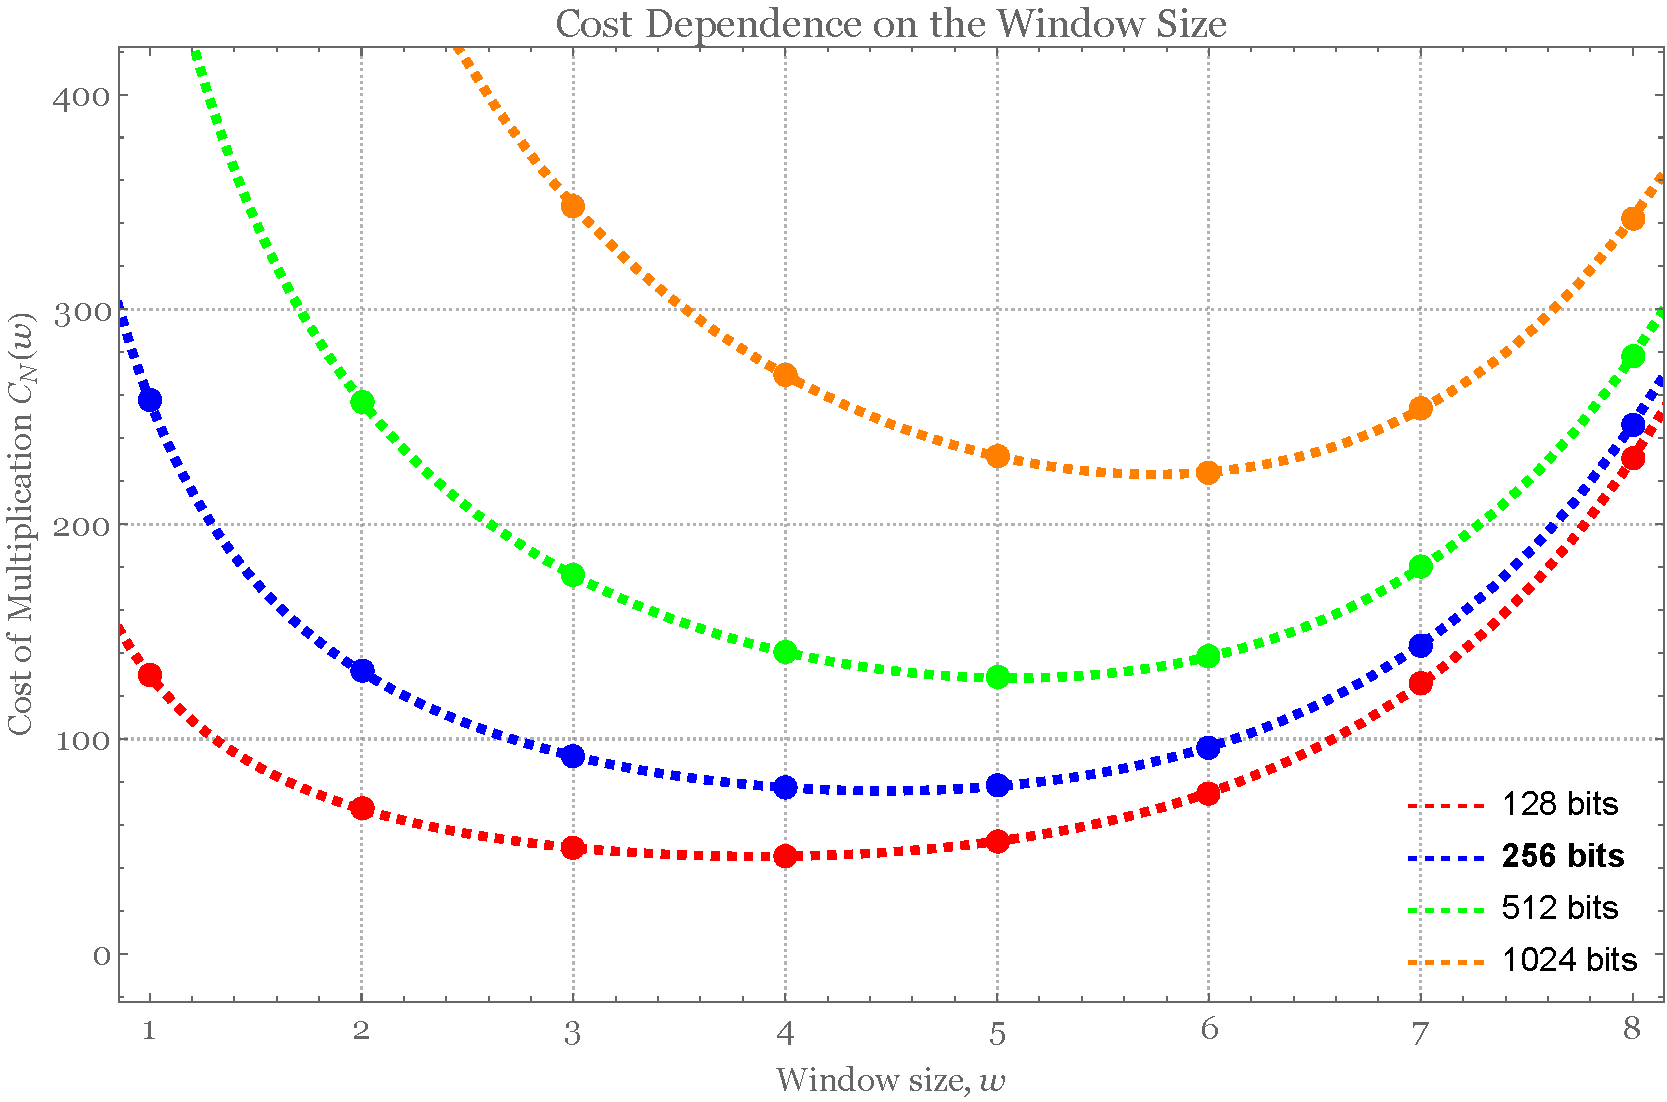
\includegraphics[width=0.75\linewidth]{window_dependence.pdf}
    \caption{Dependence of multiplication cost $C_N(w)$ on the window size $w$ for various integer bit-sizes ($N$). We plotted the dependence for four integers: \textbf{\textcolor{red}{128 bits}}, \textbf{\textcolor{blue}{256 bits}}, \textbf{\textcolor{green}{512 bits}}, \textbf{\textcolor{orange}{1024 bits}}. The dashed line in \textbf{\textcolor{blue}{blue}} is most closely related to our case ($N=254$). Here, we assumed that $C_{\mathsf{D}}/C_{\mathsf{A}} \approx 0.675$, corresponding to our multiplication.}
    \label{fig:w_dependence}
\end{figure}

\subsection{Performance Comparison}

Now, we compare our implementation with the state-of-the-art approaches currently used. To our knowledge, implementations include:
\begin{enumerate}
    \item \textit{BitVM ``Overflow'' Multiplication}\footnote{\url{https://github.com/BitVM/BitVM}, Accessed: 25 July 2024}: BitVM provides the default library to operate with big integers (thereafter, called \texttt{bigint}) that implements the \texttt{mul} operation. The catch is that, based on two $N$-bit integers, this function also returns a $N$-bit integer, reduced modulo $2^N$ (essentially, the lower limb in $2N$-bit integer representation $c_0 + c_1 \times 2^N$) --- we call this ``overflow multiplication''. Therefore, for comparison, we adapted algorithm \Cref{alg:script_windowed} to have the same functionality, and also tweaked the \textit{BitVM}'s implementation to give the $2N$-bit integer as the result.
    \item \textit{Cmpeq's Implementation}\footnote{
    \url{https://bitcointalk.org/index.php?topic=5477449.0}, Accessed: 25 July 2024}: quite recently, on Bitcoin Forum, \textit{cmpeq} claimed to have roughly \textsf{100k} opcodes in his multiplication of two $255$-bit integers. The result is a $510$-bit integer, compared to \texttt{bigint} multiplication from \textit{BitVM}. 
    \item \textit{BitVM $29\times 9$ Karatsuba Multiplication}: This is the most recent version that BitVM mostly relies on that uses the Karatsuba multiplication (see \Cref{section:karatsuba}) with $(n=29,\ell=9)$ to represent a $254$-bit integer.
\end{enumerate}

The comparison results are depicted in \Cref{tab:comparison}.

\begin{table}
\centering
\begin{tabular}{ccc} 
\hline
\textbf{Approach} & \textbf{Overflowing Multiplication} & \textbf{Widening Multiplication} \\ \Xhline{3\arrayrulewidth}
  \textbf{Cmpeq} & N/A & \num[group-separator={,}]{201879} \\ \hline
  \textbf{BitVM \texttt{bigint}} & \num[group-separator={,}]{106026} & \num[group-separator={,}]{200334} \\ \hline
 \textbf{BitVM Karatsuba} & N/A & 	
    \num[group-separator={,}]{74907} \\ \hdashline
  \textbf{Our $w$-width method} & \num[group-separator={,}]{55710} & \num[group-separator={,}]{71757} \\ 
\Xhline{3\arrayrulewidth}
\end{tabular}
\caption{Comparison of our method with the current state-of-the-art. N/A means ``non-applicable'': that is, the algorithm is not adapted to the corresponding type of task.}
\label{tab:comparison}
\end{table}

Some comments about the achieved results:
\begin{enumerate}
    \item Although Cmpeq claimed to have roughly \textsf{100k} opcodes, after uploading the script, it appears that the real number of opcodes is, in fact, \textsf{200k}. This probably happens because pushing a single integer to the stack does not always cost one opcode. For example, pushing $10^3$ costs 3 opcodes while $10^5$ costs 4.
    \item Our algorithm outperforms current multiplication methods for both overflowing and widening versions.
    \item As mentioned before, original BitVM's \texttt{bigint} does not support the widening version, so we extended the used approach (namely, double-and-add method from \Cref{alg:double_and_add}) to handle $2N$-bit result.
\end{enumerate}

\subsection{Future Directions}

Most likely, our current version is not best-optimized. In particular, we list what can help to possibly reduce the number of opcodes even further:
\begin{enumerate}
    \item Small polishes in gadgets used underneath (extending big integers to handle larger limbs, more effective addition or doubling, etc.).
    \item We have not achieved any boost using NAF methods, but that does not mean these methods are not applicable: it is curious whether something can be achieved with them. In particular, $w$-NAF form might possibly decrease the number of additions from $\frac{N}{w}$ to $\frac{N}{w+1}$ and the cost of precomputing values. On the other hand, this would require implementing subtraction and sign handling, which might be troublesome.
    \item Using different bases: we achieved the best results using 30-bit limbs to represent an integer, but maybe smaller limbs might result in something more effective.
\end{enumerate}

% --- References ---
\bibliographystyle{plain} 
\bibliography{refs} 

\end{document}
